\documentclass[11pt]{article}
\usepackage[utf8]{inputenc}
\usepackage{graphicx, mathtools, caption}
\usepackage{subcaption, listing}
\usepackage{amsmath, algorithm}
\usepackage[noend]{algpseudocode}

\topmargin -0.5in
\oddsidemargin -0.0in
\evensidemargin -0.0in
\textheight 9in
\textwidth 6.5in

\title{Python Implementation of Conway's Game of Life}
\author{Brad Green \& Edwin Weill}
\date{November 29, 2016}

\begin{document}
\maketitle

\section{Introduction}
The overall idea behind this project is to design a system that simulates \textit{Conway's Game of Life}, a cellular automaton.  The Game of Life is atypical, because this particular "game" is a zero-player game.  This means that it "plays" through evolutions without any interaction with a player.  The only interaction the player has with the system is configuring the initial state and then allowing the system evolve over time.
\par
The game is played on a two-dimensional grid of squares called \textit{cells}.  Each cell is categorized as either \textit{alive} or \textit{dead} at a particular "generation" of the simulation.  Each subsequent generation is determined by the interaction between neighbors (each cell interacts with its eight surrounding neighbors).  There are many rule variations that change the behavior of the system (i.e. how cells are spawned and how cells die).  The following set of rules is based on a rule variation known as B3/S23 (born with 3 neighbors, survive with 2 or 3 neighbors):
\begin{itemize}
	\item \textbf{Rule 1}: A living cell with fewer than 2 living neighbors dies (under-population)
	\item \textbf{Rule 2}: A living cell with 2 or 3 living neighbors lives to next generation
	\item \textbf{Rule 3}: A living cell with more than 3 living neighbors dies (over-population)
	\item \textbf{Rule 4}: A dead cell with 3 neighbors becomes alive (reproduction)
\end{itemize}

\section{Literature Review}

\section{Implementation}
The initial implementation simply uses the rules described above (or a similar rule strategy) to determine each generation as the evolution of the system and makes updates based on each cell's neighbors.  The implementation iterates through every cell in the grid (alive or dead) and determines its next state based on the rules and the state of their neighbors.  The psuedocode in Algorithm \ref{naive_conway} illustrates this "naïve" algorithm implementation:
\begin{algorithm}
	\caption{Naïve Implementation Conway's Game of Life}\label{naive_conway}
	\begin{algorithmic}[1]
		\Procedure{Naive Conway}{$width, height, cell\_initialization, max\_iterations$}
			\State $grid\gets initialize\_grid(cell\_initialization)$
			\State $count\gets 0$
			\While{$count < max\_iterations$}\Comment{Update until limit reached}
				\If{$no\ change\ from\ previous\ generation$}
					\State exit
				\EndIf
				\State $count\gets count+1$
				\For{$y < grid\_height$}
					\For{$x < grid\_width$}
						\If{$cell\ is\ living$}
							\If{$cell\ has\ 2\ or\ 3\ neighbors$}
								\State $cell.state\gets dead$
							\EndIf
						\Else
							\If{$cell\ has\ 3\ neighbors$}
								\State $cell.state\gets alive$
							\EndIf
						\EndIf
					\EndFor
				\EndFor
			\EndWhile\label{naiveendwhile}
		\EndProcedure
	\end{algorithmic}
\end{algorithm}

\section{Optimizations}
The above implementation is rather simplistic and therefore it does not perform well for larger board sizes.  The naive implementation is of computational order O(width*height) which means that every cell must be visited during each evolution between generations.  This is highly inefficient when the board size gets large, therefore leading to much longer execution times.  For this reason, optimizations need to be employed utilizing various data structures to alleviate the need to "visit" every cell in the grid.
\subsection*{Set of Living Cells}
The first optimization technique makes use of an additional set which holds all currently living cells.  The strategy only checks these cells and all 8 of their neighbors to evolve to the next generation.  For each cell, we keep a count of how many cells it touches, which can be used to check the rules and add cells to the new \textit{living} list.  This implementation is much more efficient as the number of rule checks is significantly decreased for most instances of a typical grid layout, leading to O(number of living cells) complexity.  As sets are implemented by hash tables in python which have O(1) access times, the overall complexity is O(number of living cells).
\subsection*{Quadtree}
The next optimization made use of a QuadTree data structure to save space.  A QuadTree is a modification of a typical tree structure that requires each node have four children or be a leaf node.  This specification allows the structure to naturally represent spatial data while requiring very little memory as only existing elements are stored in the tree, as opposed to an array that must be large enough for all elements.  We use the QuadTree to represent the structure of living cells, meaning every leaf node of the structure represents a living cell in the Game of Life grid.  Sets are used, much like in the first optimization, to maintain performance while saving space during evolution.  As this is a tree structure, the depth of any leaf is O(log(n)) and inserting nodes takes O(log(n)) time.  This leads to worst case performance of O(log(n) * living cells)   Figure \ref{fig:quadtree_lws} shows a representation of a Game of Life grid stored in a QuadTree.
\begin{figure}[!ht]
	\centering
	\begin{subfigure}{\textwidth}
		\centering
  	  	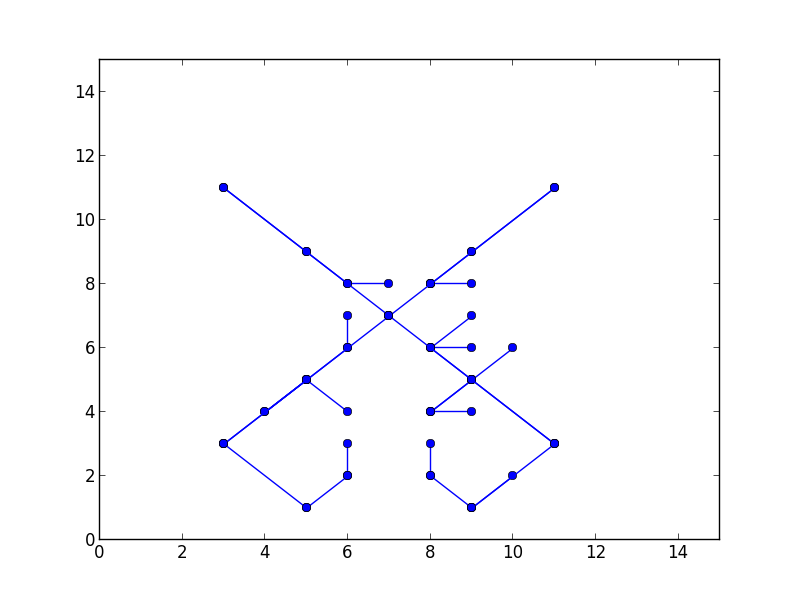
\includegraphics[width=1\linewidth]{images/quadtree_lws.png}
  	  	\label{fig:quad_lws}
	\end{subfigure}
	\caption{QuadTree Representation of Lightweight Spaceship}
	\label{fig:quadtree_lws}
\end{figure}
\section{Results}
\subsection{Visualization Results}
There are many different patterns that the game of life lends itself to when started in certain configurations.  For example, there are some patterns which do not change from one generation to the next, called still lifes.  There are others that oscillate between a set number of states; these patterns are called oscillators.  Figure \ref{fig:still} illustrates a \textit{box} which is an example of a still life while Figure \ref{fig:oscillator} illustrates a pattern with a period (an oscillator).
\begin{figure}[!ht]
	\centering
	\begin{subfigure}{.45\textwidth}
		\centering
  	  	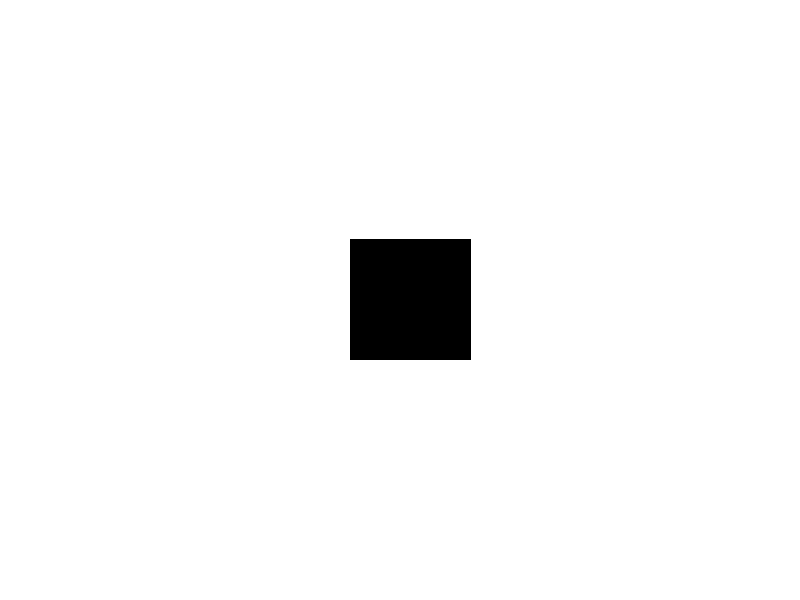
\includegraphics[width=1\linewidth]{images/box.png}
  	  	\label{fig:box1}
	\end{subfigure}
	\begin{subfigure}{.45\textwidth}
  	  	\centering
  	  	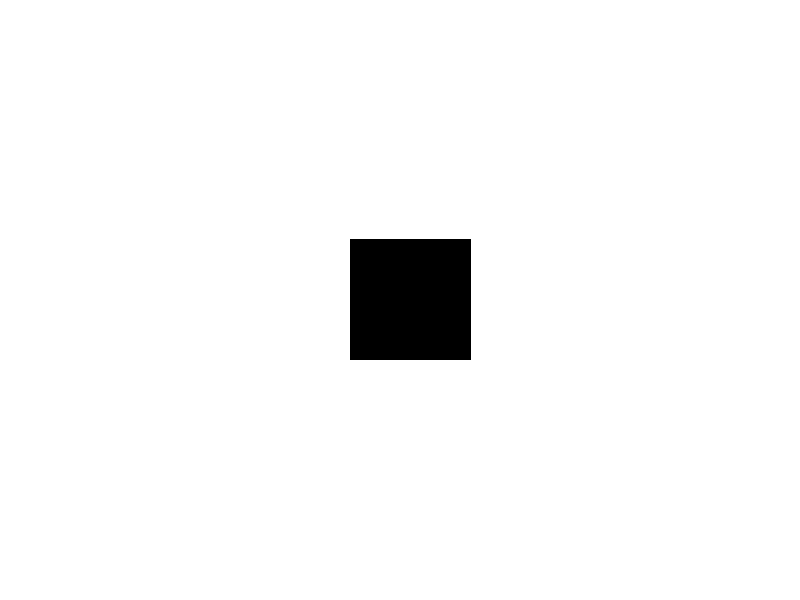
\includegraphics[width=1\linewidth]{images/box.png}
  	  	\label{fig:box2}
	\end{subfigure}
	\caption{Still Positions 1 \& 2}
	\label{fig:still}
\end{figure}

\begin{figure}[!ht]
	\centering
	\begin{subfigure}{.45\textwidth}
		\centering
  	  	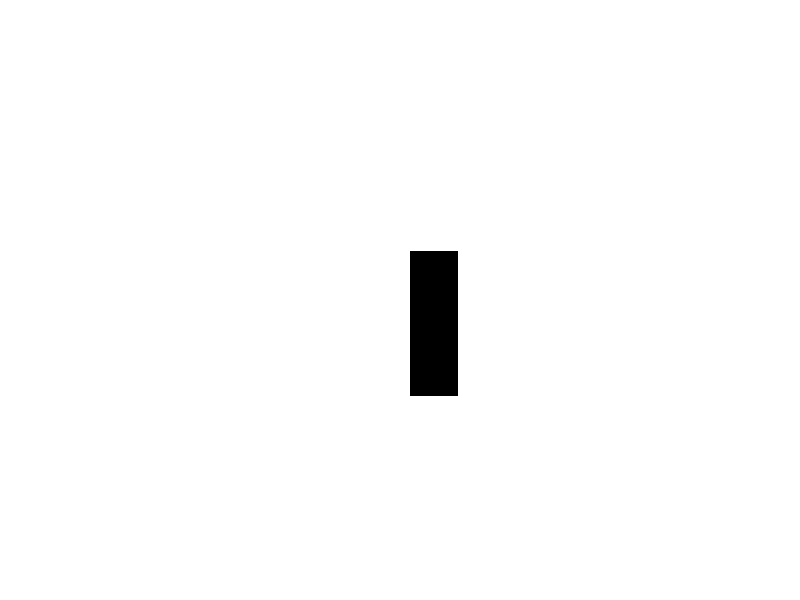
\includegraphics[width=1\linewidth]{images/blinker1.png}
  	  	\label{fig:blinker1}
	\end{subfigure}
	\begin{subfigure}{.45\textwidth}
  	  	\centering
  	  	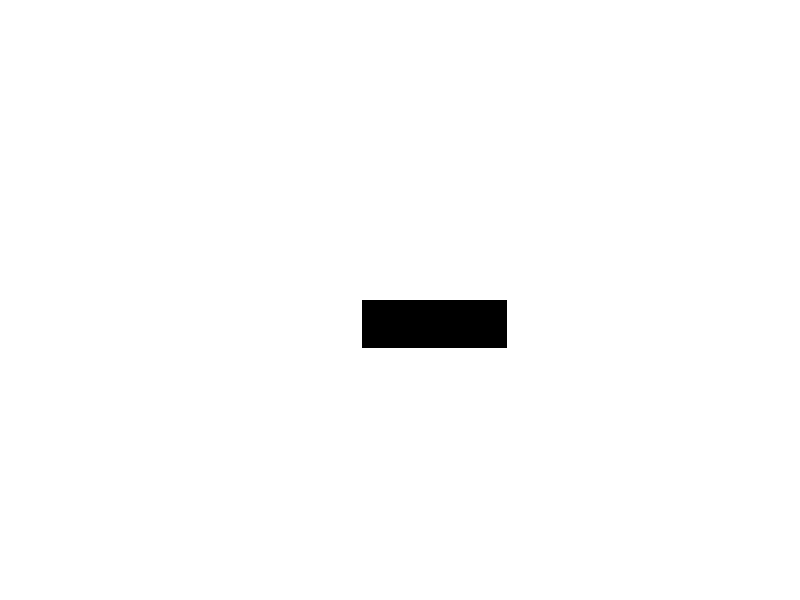
\includegraphics[width=1\linewidth]{images/blinker2.png}
  	  	\label{fig:blinker2}
	\end{subfigure}
	\caption{Oscillator Positions 1 \& 2}
	\label{fig:oscillator}
\end{figure}

There are many other types of patterns that facilitate good visualizations including glider guns (shown in Figure \ref{fig:glider_gun}).  The glider is created from the \textit{gun} every 30 iterations based on the B3/S23 rule strategy.  Another interesting example is a single live cell beginning the game with the automaton B1/S12 resulting in a very close approximation of the Sierpinski triangle.  Figure \ref{fig:sierpinski_triangle} illustrates this example.

\begin{figure}[!ht]
	\centering
	\begin{subfigure}{.45\textwidth}
		\centering
  	  	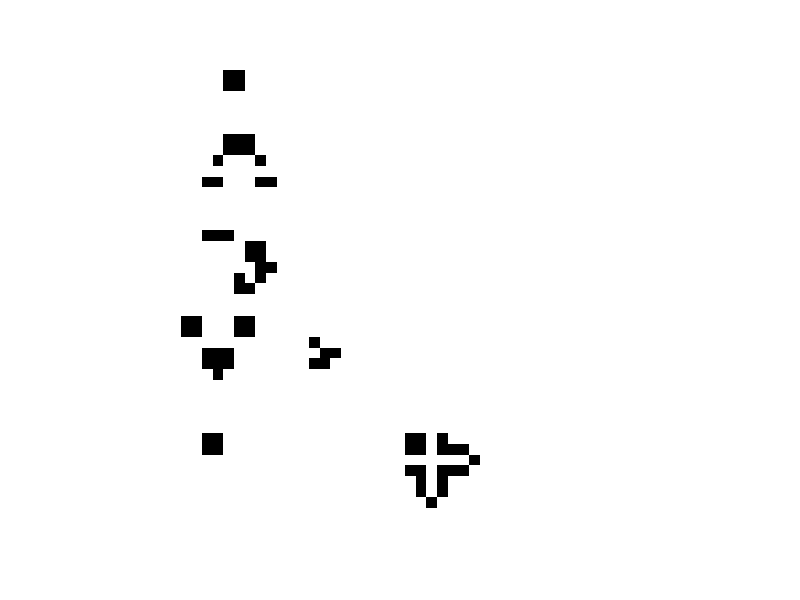
\includegraphics[width=1\linewidth]{images/glider_gun1.png}
  	  	\label{fig:glider_gun1}
	\end{subfigure}
	\begin{subfigure}{.45\textwidth}
  	  	\centering
  	  	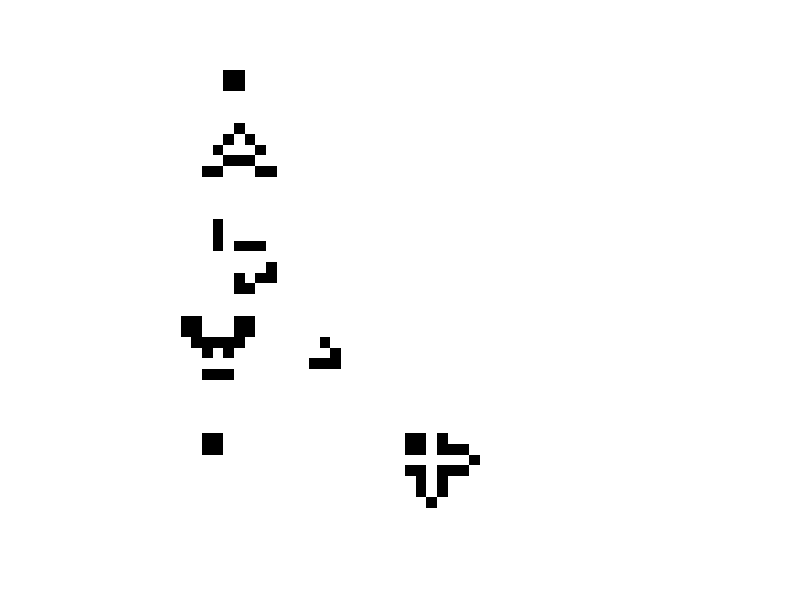
\includegraphics[width=1\linewidth]{images/glider_gun2.png}
  	  	\label{fig:glider_gun2}
	\end{subfigure}
	\caption{Glider Gun Positions 1 \& 2}
	\label{fig:glider_gun}
\end{figure}

\begin{figure}[!ht]
	\centering
	\begin{subfigure}{\textwidth}
		\centering
  	  	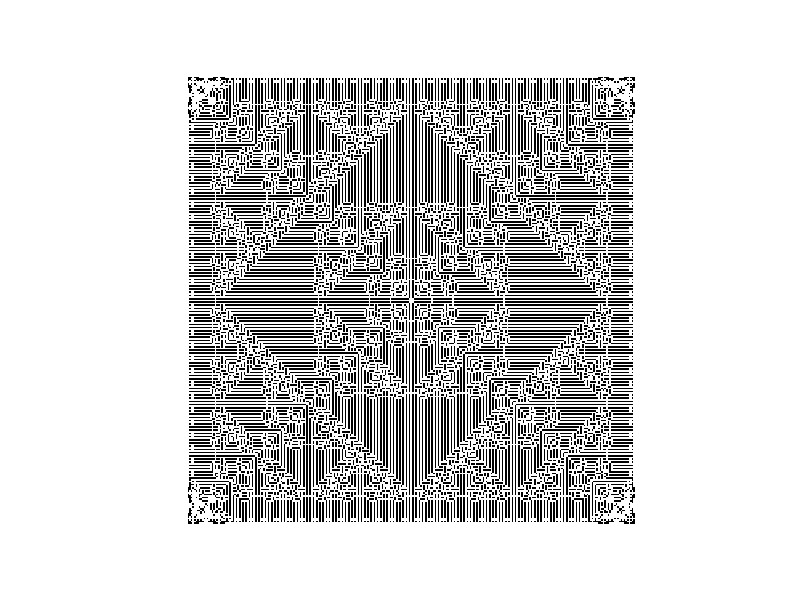
\includegraphics[width=1\linewidth]{images/sierpinski.png}
  	  	\label{fig:sierpinski1}
	\end{subfigure}
	\caption{Sierpinski Triangle}
	\label{fig:sierpinski_triangle}
\end{figure}

\subsection{Performance Results}
To compare the methods, we created a Game of Life grid with set initial conditions (each cell has a 30\% chance to start as alive) to verify all methods completed the same evolutions.  100 generations were simulated for each method using the B3/S23 ruleset.  Figure \ref{fig:avg_mem_use} shows the memory taken by the different optimization methods for growing grid sizes.  Figure \ref{fig:avg_time_use} shows the time taken by each method for the same test conditions.
\begin{figure}[!ht]
	\centering
	\begin{subfigure}{\textwidth}
		\centering
  	  	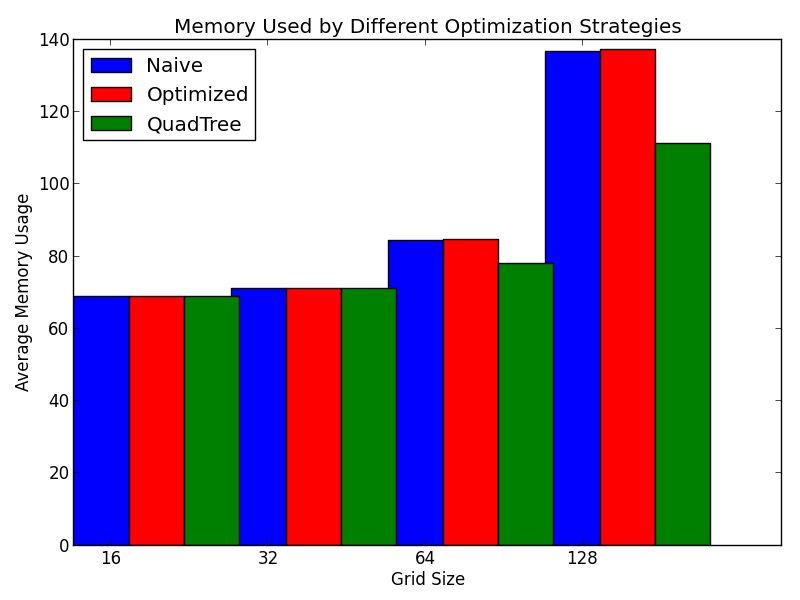
\includegraphics[width=1\linewidth]{images/average_random.png}
  	  	\label{fig:avg_mem}
	\end{subfigure}
	\label{fig:avg_mem_use}
\end{figure}
\begin{figure}[!ht]
	\centering
	\begin{subfigure}{\textwidth}
		\centering
  	  	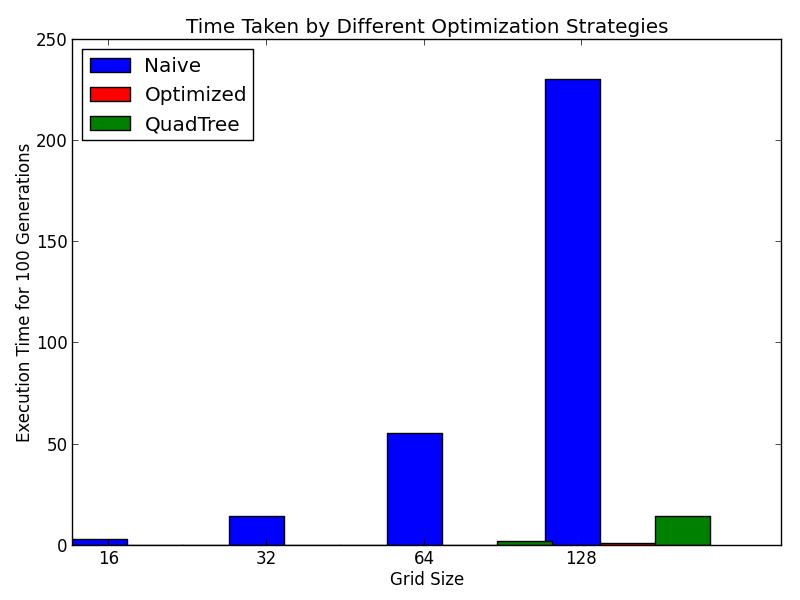
\includegraphics[width=1\linewidth]{images/time_random.png}
  	  	\label{fig:avg_time}
	\end{subfigure}
	\label{fig:avg_time_use}
\end{figure}
\section{Discussion}
As shown in Figure \ref{fig:avg_mem_use}, the QuadTree implementation used less memory than both the Naive and Optimized methods as only alive nodes are saved.  The graph represents the memory usage of the entire python program, including all overhead for imported modules.  If we take the 16x16 grid as a baseline and normalize the 128x128 grid to this, we can see the QuadTree implementation saves significant memory over the other methods to store the Game of Life grid.  Further, the tested version of the QuadTree does not \textit{prune} empty branches to save on time, so there is an added overhead of empty branches stored in the tree.  Figure \ref{fig:avg_time_use} shows that our optimized version runs fastest due to the constant access times of the hash tables for the sets.  If we were to prune the QuadTree, it would take significantly longer to run (pruning recursively checks all branches and deletes any which have no leaves).
\section{Distribution of Work}

\end{document}
